\documentclass[a4paper]{article}
\usepackage[utf8]{inputenc}
\usepackage{amsmath}
\usepackage{amssymb}
\usepackage{caption}
\usepackage{mathtools}
\usepackage{amsfonts}
\usepackage{lastpage}
\usepackage{tikz}
\usepackage{float}
\usepackage{textcomp}
\usetikzlibrary{patterns}
\usepackage{pdfpages}
\usepackage{gauss}
\usepackage{fancyvrb}
\usepackage[table]{colortbl}
\usepackage{fancyhdr}
\usepackage{graphicx}
\usepackage[margin=2.5 cm]{geometry}

\definecolor{listinggray}{gray}{0.9}
\usepackage{listings}
\lstset{
	language=,
	literate=
		{æ}{{\ae}}1
		{ø}{{\o}}1
		{å}{{\aa}}1
		{Æ}{{\AE}}1
		{Ø}{{\O}}1
		{Å}{{\AA}}1,
	backgroundcolor=\color{listinggray},
	tabsize=3,
	rulecolor=,
	basicstyle=\scriptsize,
	upquote=true,
	aboveskip={0.2\baselineskip},
	columns=fixed,
	showstringspaces=false,
	extendedchars=true,
	breaklines=true,
	prebreak =\raisebox{0ex}[0ex][0ex]{\ensuremath{\hookleftarrow}},
	frame=single,
	showtabs=false,
	showspaces=false,
	showlines=true,
	showstringspaces=false,
	identifierstyle=\ttfamily,
	keywordstyle=\color[rgb]{0,0,1},
	commentstyle=\color[rgb]{0.133,0.545,0.133},
	stringstyle=\color[rgb]{0.627,0.126,0.941},
  moredelim=**[is][\color{blue}]{@}{@},
}

\lstdefinestyle{base}{
  emptylines=1,
  breaklines=true,
  basicstyle=\ttfamily\color{black},
}

\pagestyle{fancy}
\def\checkmark{\tikz\fill[scale=0.4](0,.35) -- (.25,0) -- (1,.7) -- (.25,.15) -- cycle;}
\newcommand*\circled[1]{\tikz[baseline=(char.base)]{
            \node[shape=circle,draw,inner sep=2pt] (char) {#1};}}
\newcommand*\squared[1]{%
  \tikz[baseline=(R.base)]\node[draw,rectangle,inner sep=0.5pt](R) {#1};\!}
\newcommand{\comment}[1]{%
  \text{\phantom{(#1)}} \tag{#1}}
\def\el{[\![}
\def\er{]\!]}
\def\dpip{|\!|}
\def\MeanN{\frac{1}{N}\sum^N_{n=1}}
\cfoot{Page \thepage\ of \pageref{LastPage}}
\DeclareGraphicsExtensions{.pdf,.png,.jpg}
\author{Nikolaj Dybdahl Rathcke (rfq695)}
\title{Signal and Image Processing \\ Assignment 6}
\lhead{SIP}
\rhead{Assignment 6}

\begin{document}
\maketitle

\section{Experiments on translations}
\subsection{}
The image $\widetilde{I}(i, j)$ which is obtained by shifting the image $I$ one pixel to the right is called a translation of $I$ and can mathematically be expressed as $\widetilde{I}(i, j)=I(i-1, j)$. The filter $h$ for the operation can be expressed as:
\begin{align*}
  h = \begin{bmatrix} 1 & 0 & 0\end{bmatrix}
\end{align*}
which, looking at one pixel, would simply only include the intesity of the pixel to the left.

\subsection{}
The code found in \texttt{src/q1\_2.m} translates an image $I$ of size $(77, 77)$ with a white square in the middle of size $3$ by $3$. It is translated with the vector $d=\begin{bmatrix} 30 \\ 30 \end{bmatrix}$ using Matlab's built-in function \texttt{imtranslate}, but the method \texttt{shiftImg} takes any parameters for $x$ and $y$. Figure \ref{fig1} show the original image and the result after translation with $d$.
\begin{figure}[H]
  \centering
  \captionsetup{justification=centering}
  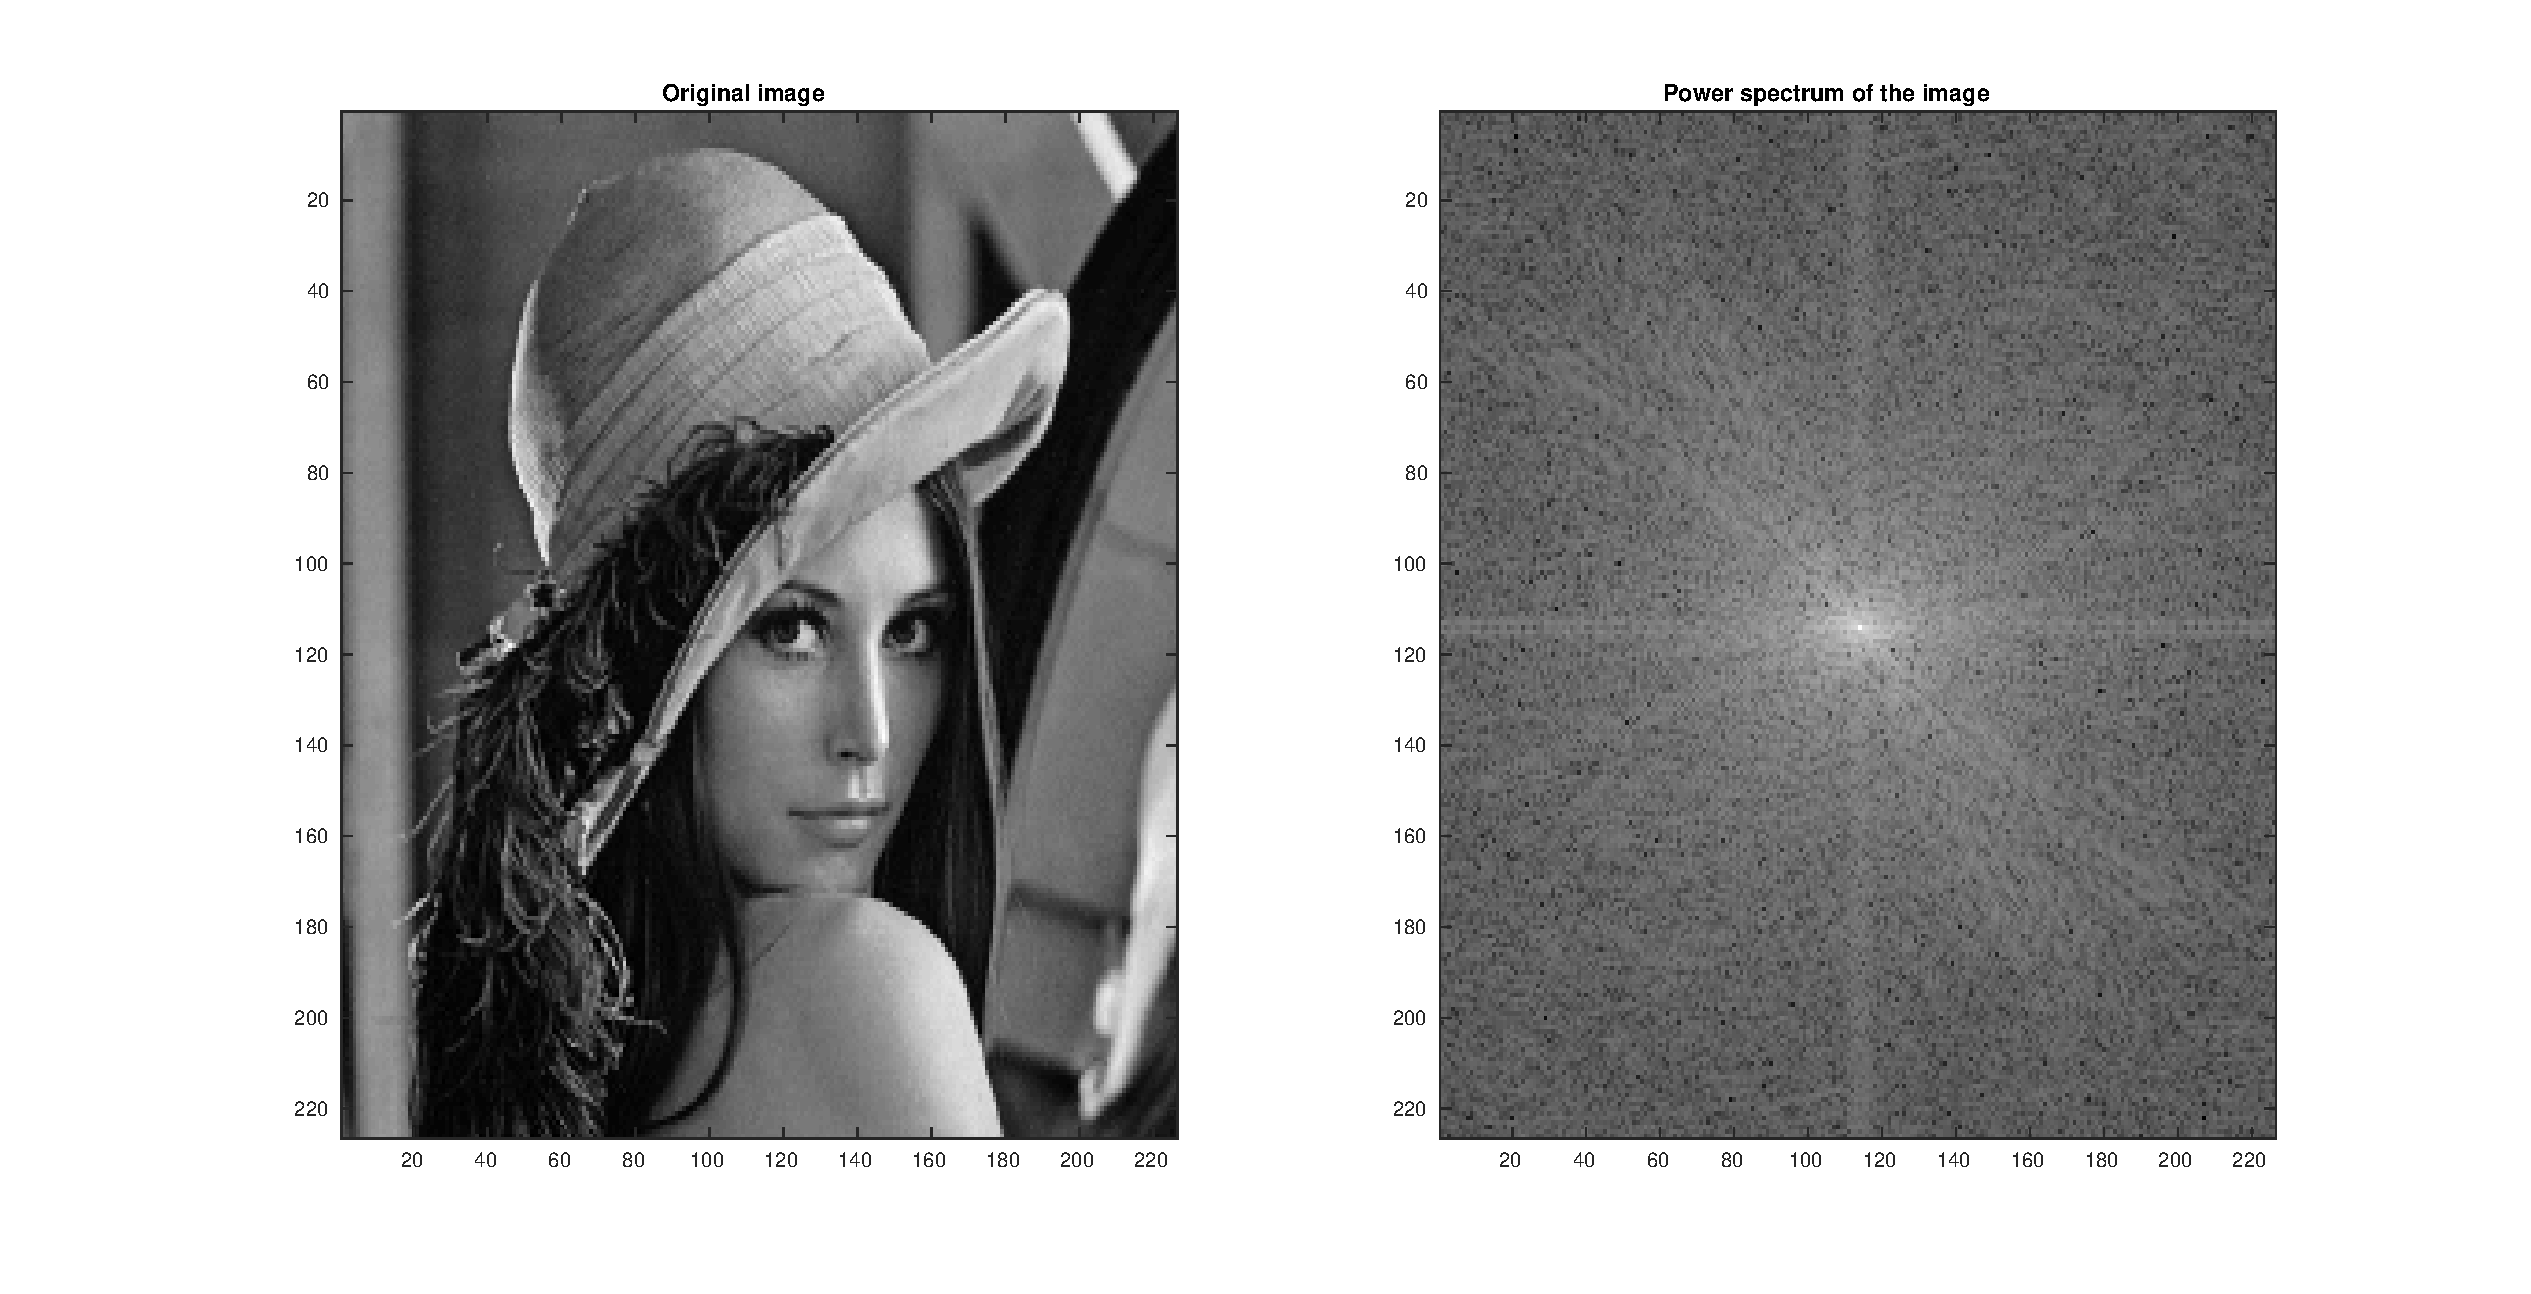
\includegraphics[width=\textwidth]{fig1.eps}
  \caption{An image I and the result after translating it with vector $d$.}
  \label{fig1}
\end{figure}
Where the image is shifted $30$ pixel along both axes. However, we need to consider that it might try to access an index which is out of bounds for $I$. To overcome this, we could extend the image with rows and columns corresponding to the given $x$ and $y$, with all values set to some constant ($0$ in this image). If the filter is constructed in the same way as (1.1), we can expect it to have size $x\cdot y$, so extending the image would ensure that the translation is possible. We would have to remove the rows and columns we added afterwards (meaning we could move the white square out of the image, so we are left with a completely black image).

\subsection{}
A property of the Fourier transform is that a shift in the time domain does not make a difference for the frequencies, but it does change the phase of the frequencies. The shift theorem states that a translation in one of the domains corresponds to a multiplication by some complex exponential in the other domain. This thought is implemented in \texttt{src/q1\_3.m} and produces Figure \ref{fig7}.
\begin{figure}[H]
  \centering
  \captionsetup{justification=centering}
  
\includegraphics[width=\textwidth]{fig7.eps}
  \caption{Comparison between using a simple translation and translation with FFT.}
  \label{fig7}
\end{figure}
As we can see, the result from using translation with FFT is exactly the same as we found in (1.2).

\subsection{}
This is possible as the translation in the frequency domain is performed by shifting the phase and this is possible for any real number. However, if we shift it with a non-integer, the phase will affect more than one pixel. Figure \ref{fig8} show the result of this.
\begin{figure}[H]
  \centering
  \captionsetup{justification=centering}
  \includegraphics[width=\textwidth]{fig8.eps}
  \caption{Comparison between integer and non-integer values when doing translations with FFT.}
  \label{fig8}
\end{figure}
As we can see, the image with translation with FFT and non-integer values is distorted as we expected.

\section{Procrustes transformations}
\subsection{}
The $2D$ Procrustes transformation has four free variables. This is because the Procrustes transformation only performs a translation $X$, a rotation $R$ and a scaling $S$. Thus, the transformation is given by $T=SRX$. The scaling has one free variable, the rotation has one free variable and the translation has two free variables, hence the four free variables. The last two free variables come from the shear transformation in affine transformations. \\
We know that to find a single solution to $n$ free variables, we need at least $n$ (different) equations. As we have points (that have two unknowns), we will need at least two points, so our minimal $N$ should be $2$.

\subsection{}
This was implemented \texttt{src/q2\_2.m}. The two images loaded in and we use Matlab's \texttt{getpts} to get the coordinates of three points for both images. The points that were chosen are located near the three big intersections. We then use \texttt{cp2tform} with the coordinates for both images and the parameter 'nonreflective similarity' as the documentation states that this option is used when the image is only distorted by translation, rotation or scaling (Procrustes). Finally, we apply the transformation using Matlab's \texttt{imtransform}. In Figure \ref{fig2}, we see the result from attempting to transform the image \texttt{westconcordaerial.png} to the image \texttt{westconcordorthophoto.png}.
\begin{figure}[H]
  \centering
  \captionsetup{justification=centering}
  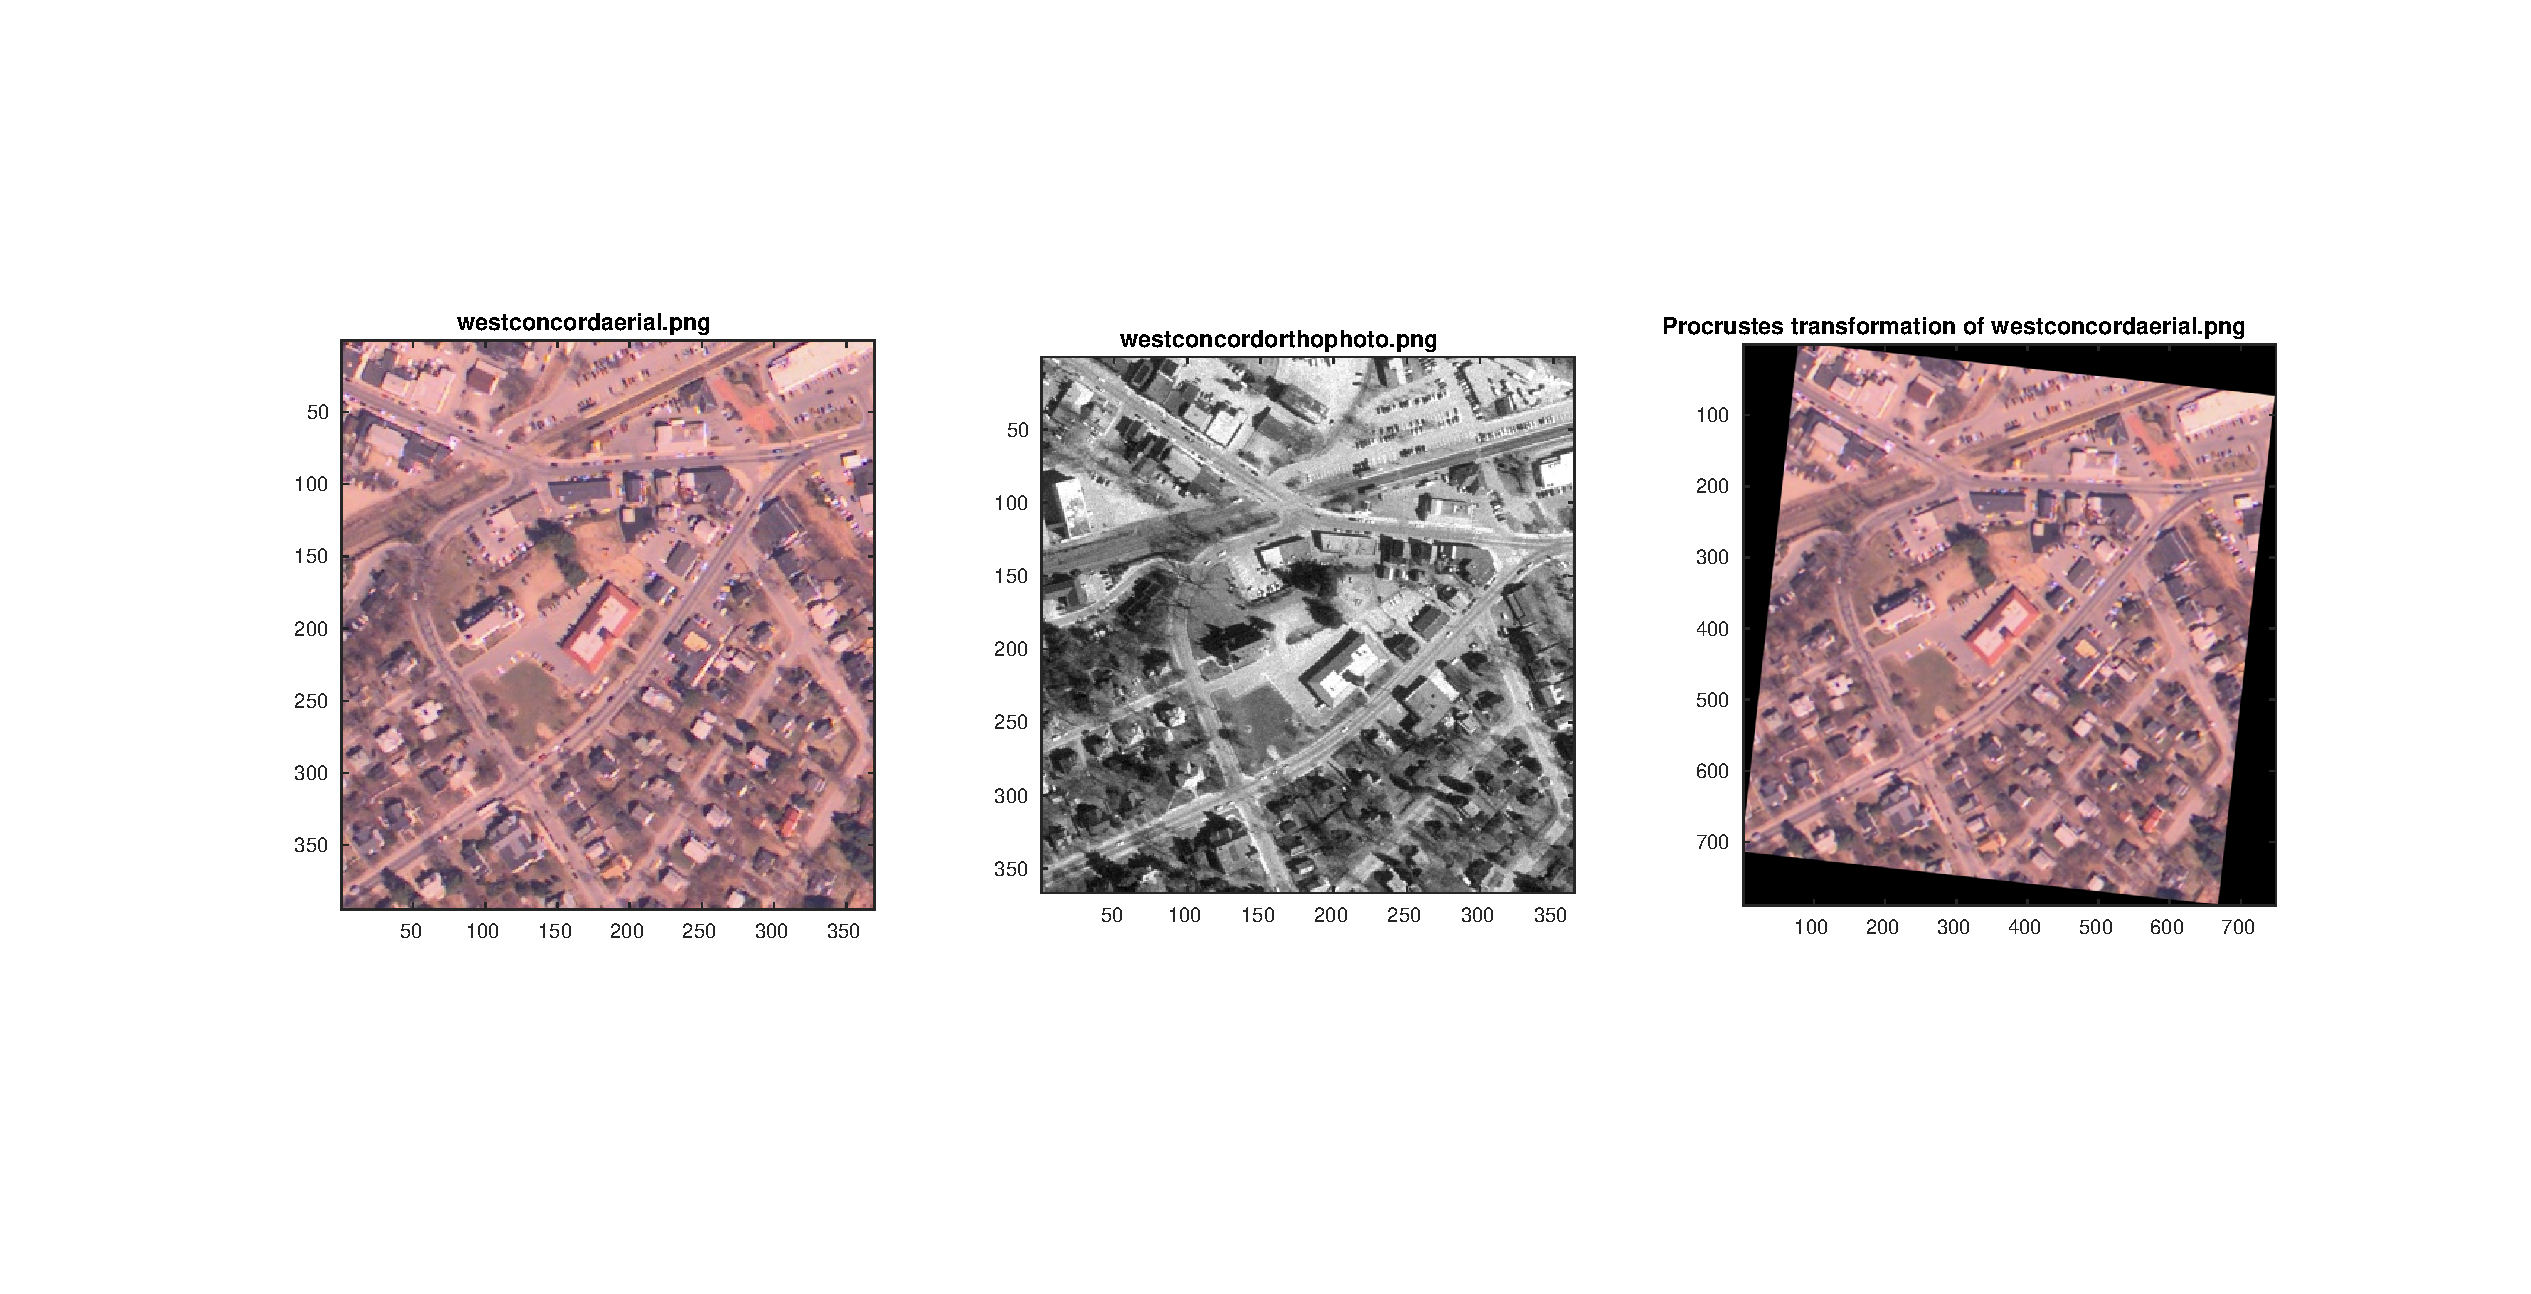
\includegraphics[width=\textwidth]{fig2.eps}
  \caption{Two images of the same location and the Procrustes transformation of the first image to make it look like the second.}
  \label{fig2}
\end{figure}
We can clearly see the image has been scaled and rotated slightly to the right to match the target image (the middle one). The translation is a bit harder to see, but the three intersections should be located in the same place as in the target. This might not be completely accurate as I think Matlab's \texttt{getpts} did not work very well with my window manager, so these could be more precise.

\section{Bonus: Optimal rotation for Procrustes alignment}
Not completed.

\section{Affine and projective alignments}
\subsection{}
The main advantage of using homogeneous coordinates is that we not need to perform a vector addition if we want to translate the image. This means that any transformation can be written as matrix multiplication which is practical as it is faster and easier. It is also more practical in the sense that if we want to perform a sequence of transformations (scaling, rotation, translation, shearing), we would like a single matrix (precomputed) that we can apply to all input. If we have translation that requires a vector addition, we are prevented from doing this.

\subsection{}
The plot of the two quadrilaterals given by $X$ and $Y$ can be seen in Figure \ref{fig3} which is produced by running the file \texttt{src/q4\_2.m}.
\begin{figure}[H]
  \centering
  \captionsetup{justification=centering}
  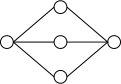
\includegraphics[width=\textwidth]{fig3.eps}
  \caption{Two quadrilaterals given by the dataset $X$ and $Y$}
  \label{fig3}
\end{figure}
There cannot be a Procrustes transformation from one quadrilateral to the other. A Procrustes transformation retains its shape as we only perform scalings, rotations and translation. If we wanted to turn one of the into the other, we would need to use shear transformations as well. \\
With the Procrustes alignment, implemented in Matlab as \texttt{procrustes}, we can try to match one quadrilateral with the other as best as we can (the one with the smallest squared error between points). Running \texttt{src/q4\_2b}, we try to scale, rotate and translate the dataset $X$. This results in Figure \ref{fig4}
\begin{figure}[H]
  \centering
  \captionsetup{justification=centering}
  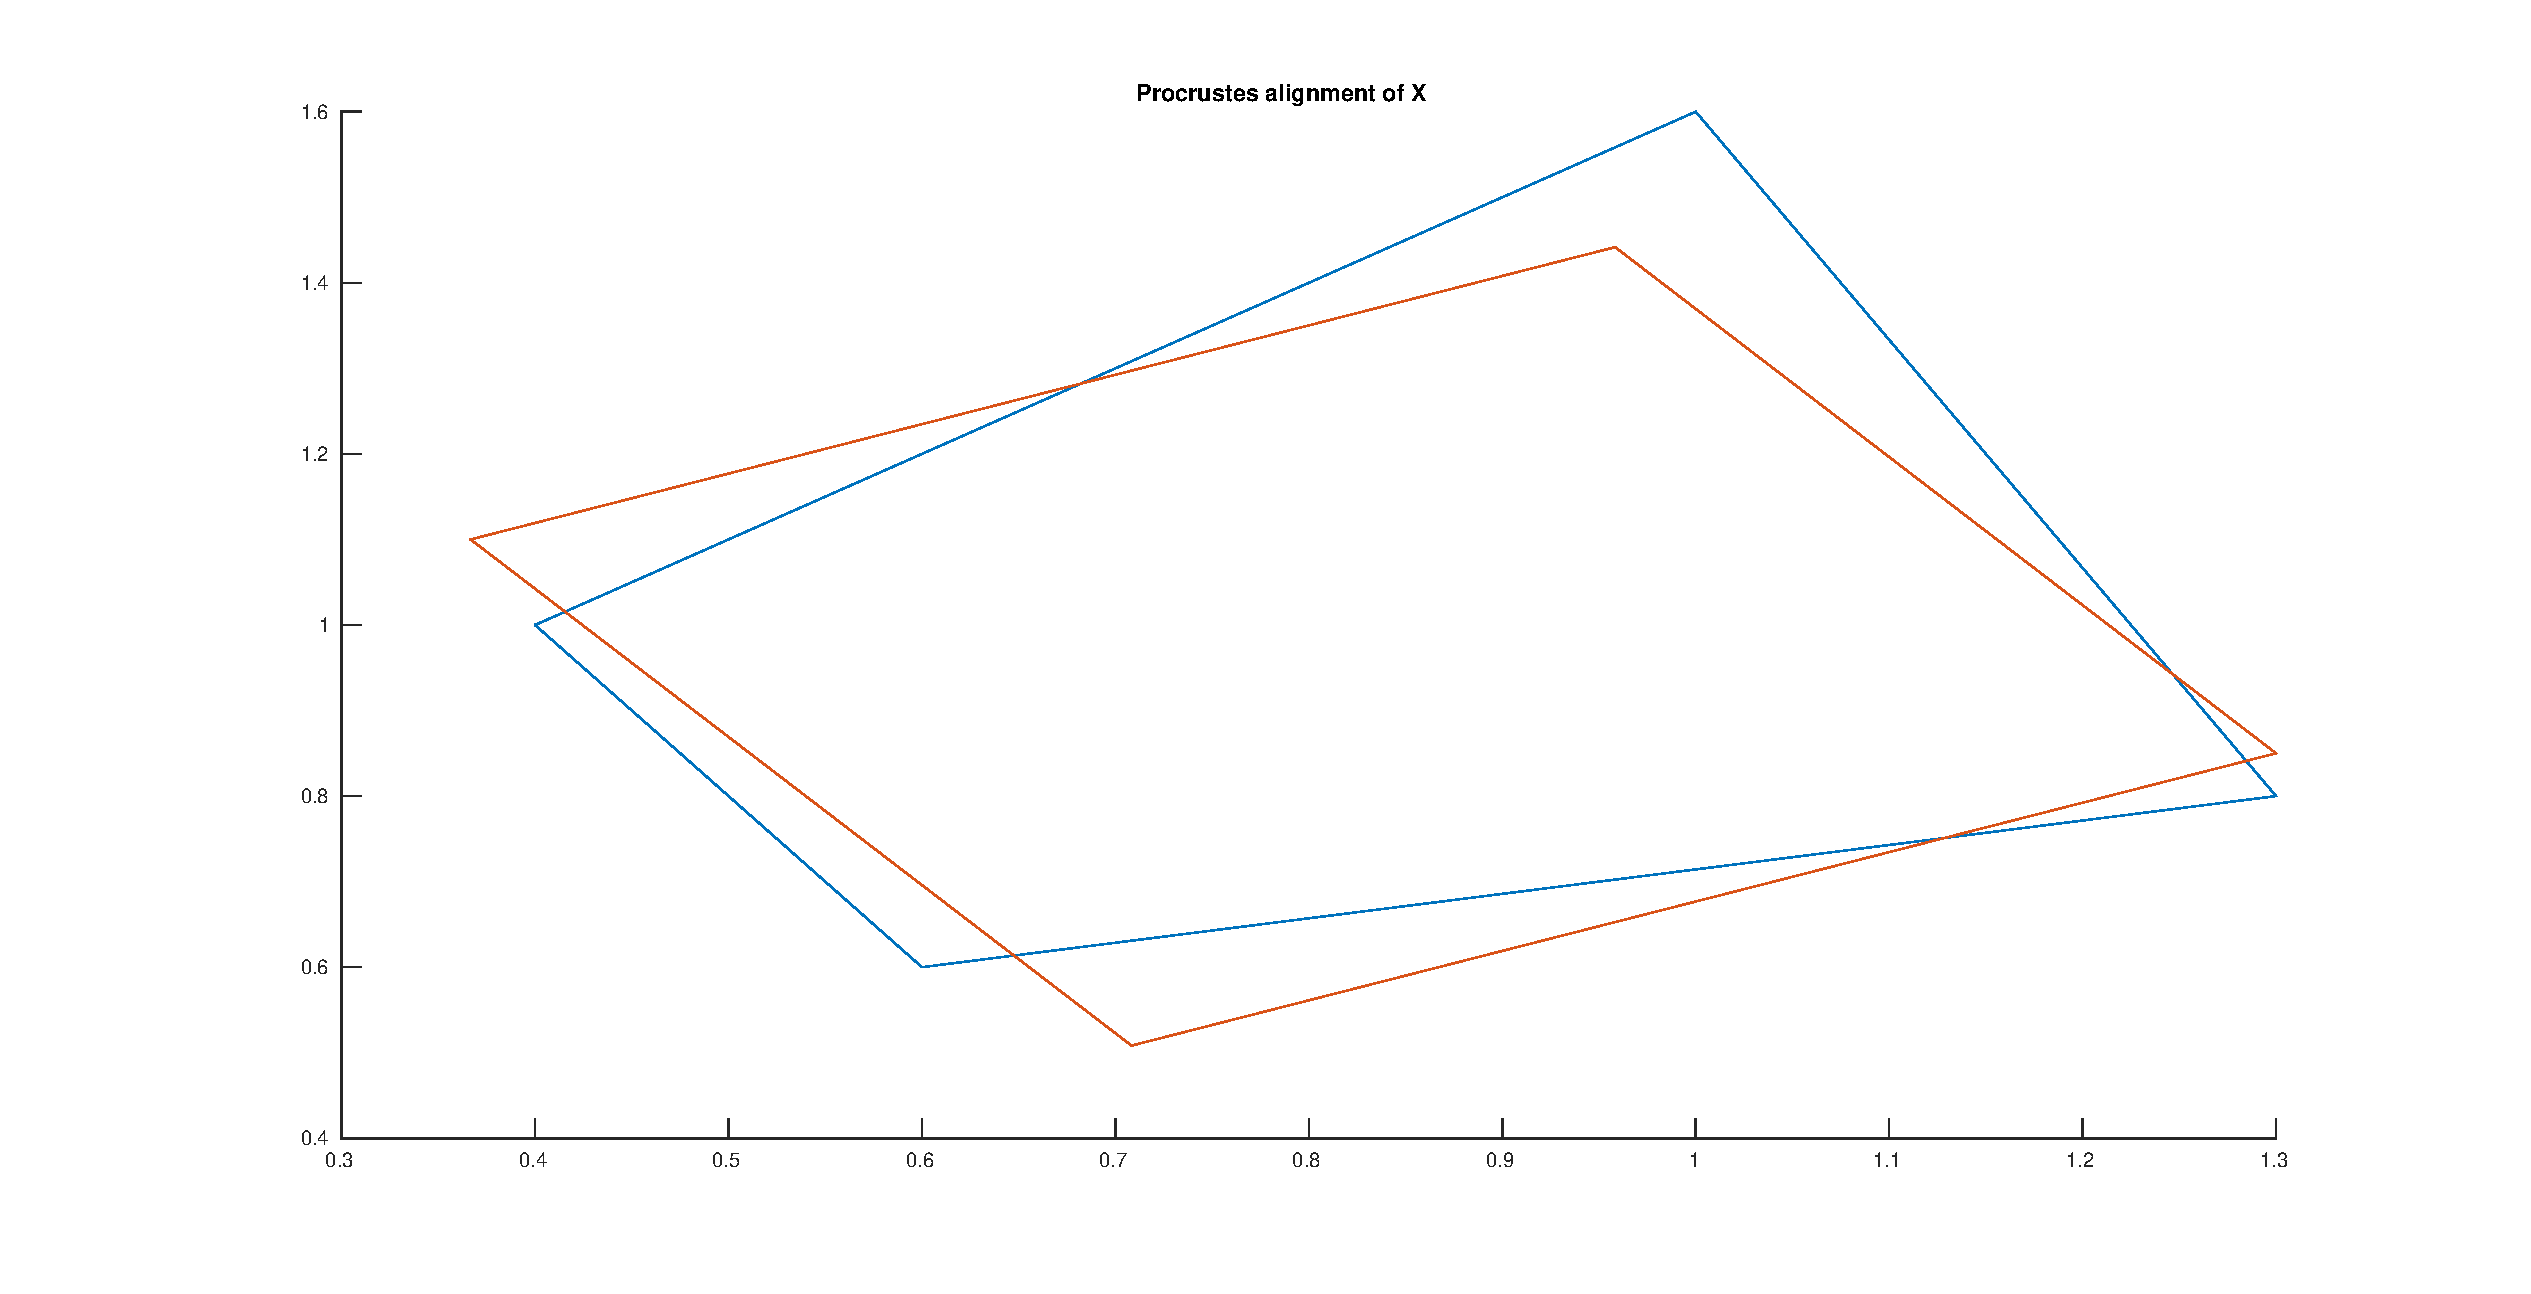
\includegraphics[width=\textwidth]{fig4.eps}
  \caption{Procrustes alignment of dataset $X$ with respect to $Y$.}
  \label{fig4}
\end{figure}
This is the best transformation we can perform on $Y$ to make it look like $X$. We can see that all three types of transformation have been used.

\subsection{}
It is not possible to make an affine transformation between the two quadrilateral in Figure \ref{fig3} even though we are also allowed to use shear transformations. This is due parallel lines remains parallel after an affine transformation. We can see the quadrilateral given by dataset $Y$ has two diagonal non-parallel lines, while all diagonal lines in the quadrilateral given by $X$ are parallel. \\
Figure \ref{fig5}, obtained by running \texttt{q4\_3.m} shows the result of trying to make an affine transformation from $X$ to $Y$.
\begin{figure}[H]
  \centering
  \captionsetup{justification=centering}
  
\includegraphics[width=\textwidth]{fig5.eps}
  \caption{Affine alignment of dataset $X$ with respect to $Y$.}
  \label{fig5}
\end{figure}
As we can see, the transformation is not perfect, which we expected. However, it is closer to a perfect transformation than for Procrustes alignment as we are allowed to do shear transformations as well.

\subsection{}
The projective transform has eight degrees of freedom. This means we have eight free variables and as we found in (2.1), that means we can make a perfect transformation for four points. Figure \ref{fig6} shows the result of projective transform implemented in \texttt{src/q4\_4.m}.
\begin{figure}[H]
  \centering
  \captionsetup{justification=centering}
  \includegraphics[width=\textwidth]{fig6.eps}
  \caption{Affine alignment of dataset $X$ with respect to $Y$.}
  \label{fig6}
\end{figure}
We can only see the dataset $Y$, because the transformation is perfect (so there are two dataset with the same points in the figure).

\end{document}
